\documentclass[a4paper, 12pt]{article}
\usepackage[UTF8]{ctex}
\usepackage{float}
\usepackage{graphicx}

\begin{document}
	\title{系统开发工具基础实验报告(四)}
	\author{22110032031 张希敏}
	\date{\today}
	\maketitle
	
	\pagenumbering{roman}
	\tableofcontents
	\newpage
	\pagenumbering{arabic}
	
	\section{练习主题}
	\paragraph{(1)调试及性能分析}
	
	\paragraph{(2)元编程演示实验}
	
	\paragraph{(3)大杂烩}
	
	\paragraph{(4)PyTorch 编程}
	
	\section{练习内容}
	
	\subsection{四个题目}
	
	\subsubsection{题目一}
	使用 Linux 上的 journalctl 或 macOS 上的 log show 命令来获取最近一天中超级用户的登录信息及其所执行的指令。
	
	\paragraph{答:}
	输入命令 journalctl | grep sudo
	
	\begin{figure}[H]
		\centering
		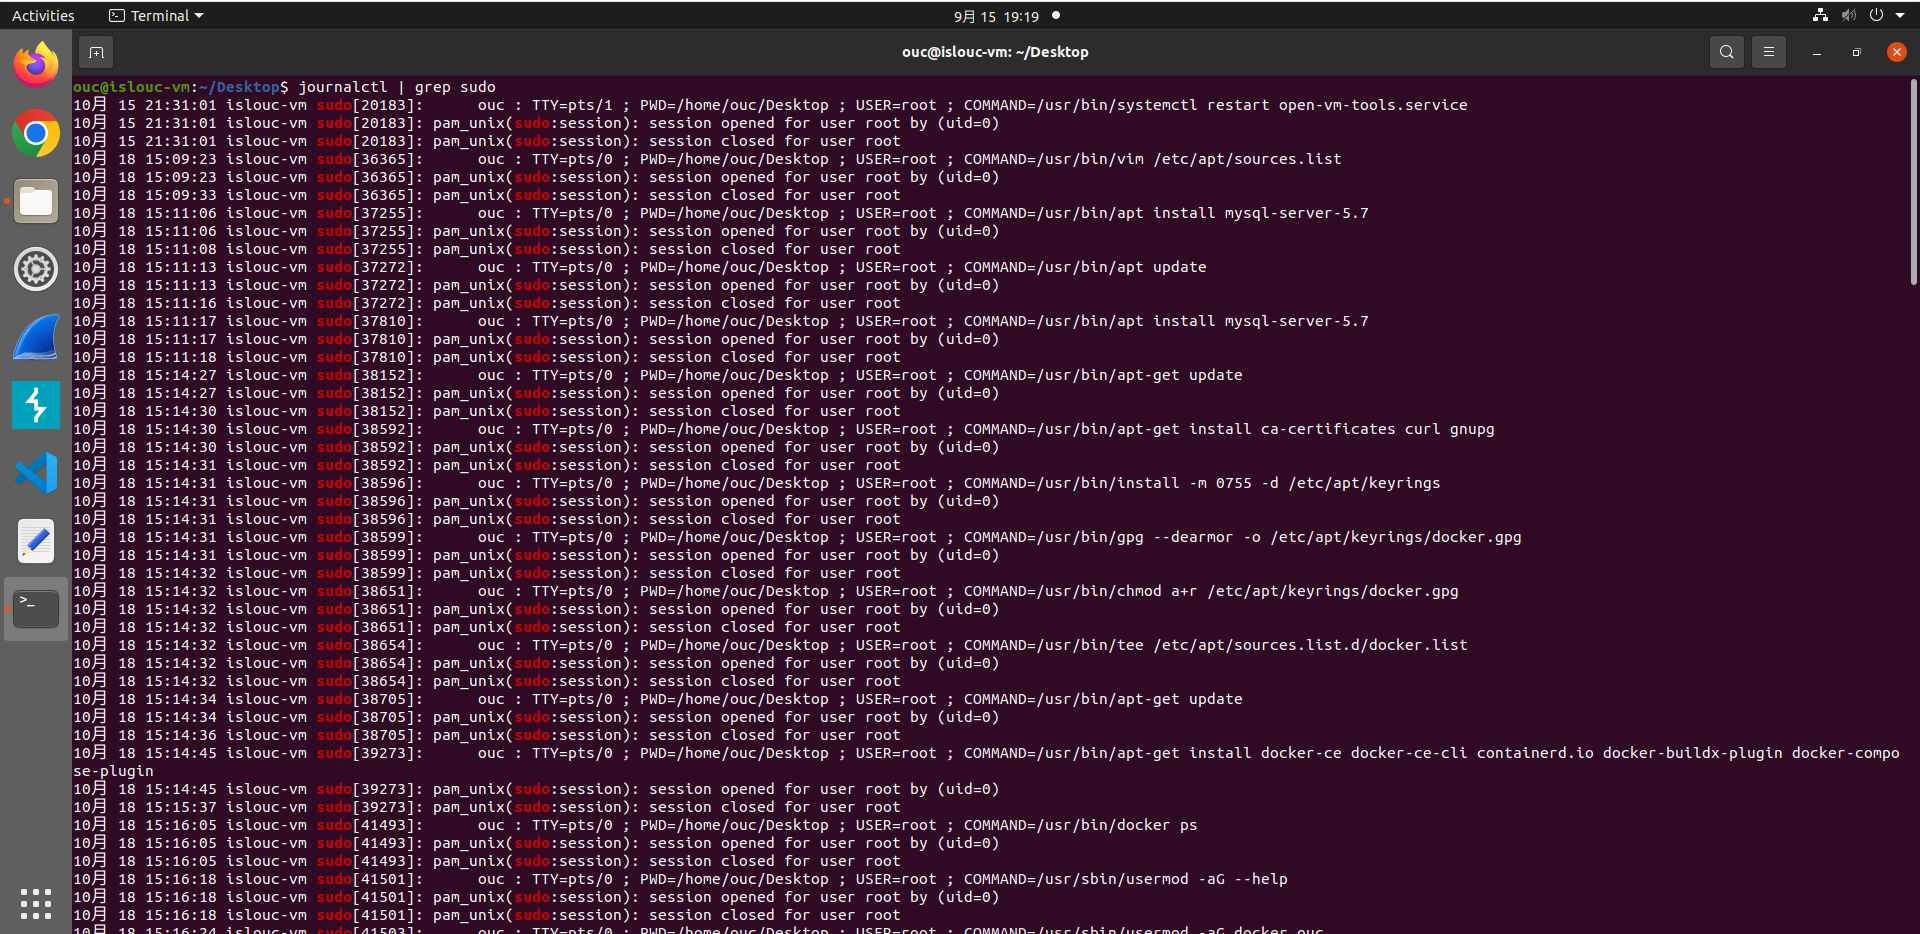
\includegraphics[width=1\textwidth]{001.jpg}
	\end{figure}
	

	\subsubsection{题目二}
	请使用 cProfile 和 line\_profiler 来比较插入排序和快速排序的性能。两种算法的瓶颈分别在哪里?然后使用 memory\_profiler 来检查内存消耗,为什么插入排序更好一些?然后再看看原地排序版本的快排。
	
	\paragraph{答:}
	使用 cProfile 按照执行时间排序,输入命令  python -m cProfile -s time sorts.py | grep sorts.py
		
	\begin{figure}[H]
		\centering
		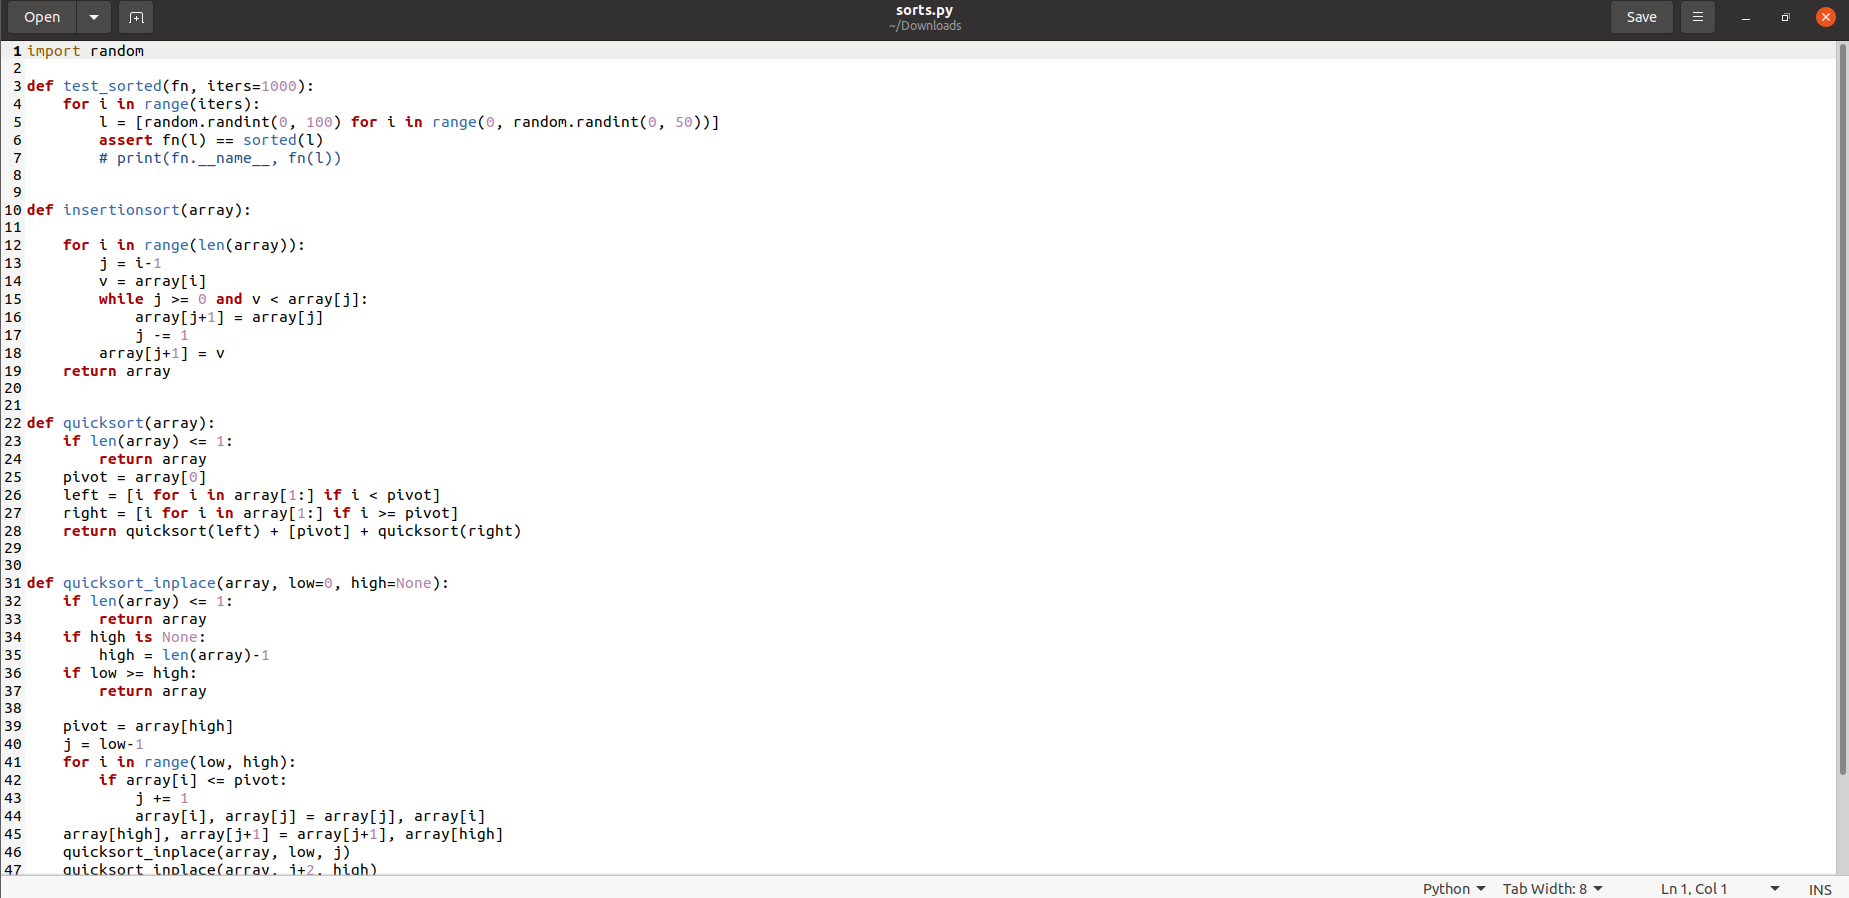
\includegraphics[width=1\textwidth]{002.jpg}
		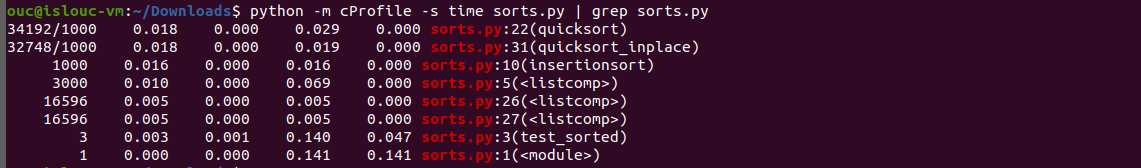
\includegraphics[width=1\textwidth]{003.jpg}
	\end{figure}
	
	使用 line\_profiler进行分析,需要安装:

	pip install line\_profiler
	
	然后为需要分析的函数添加装饰器 @profile,并执行:
	
	kernprof -l -v sorts.py
	
	结果如图:
	
	\begin{figure}[H]
		\centering
		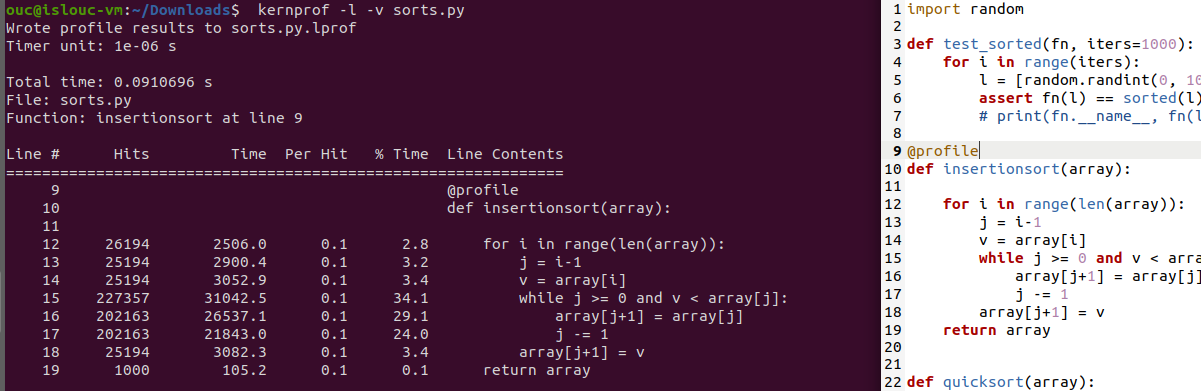
\includegraphics[width=1\textwidth]{004.jpg}
		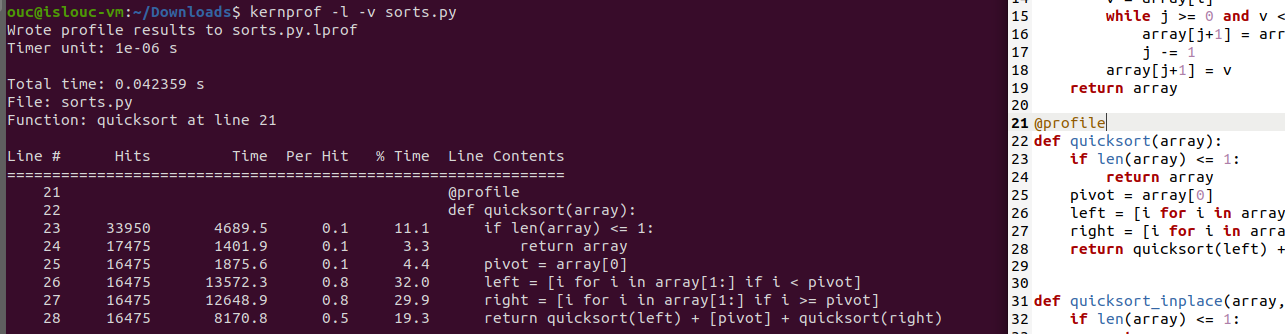
\includegraphics[width=1\textwidth]{005.jpg}
	\end{figure}
	
	插入排序的耗时更高一些。快速排序的瓶颈在于 left和 right的赋值,而插入排序的瓶颈在while循环。
	
	使用 memory\_profiler进行分析,需要安装:
	
	pip install memory\_profiler
	
	同样需要添加@profile 装饰器。结果如图:
	
	\begin{figure}[H]
		\centering
		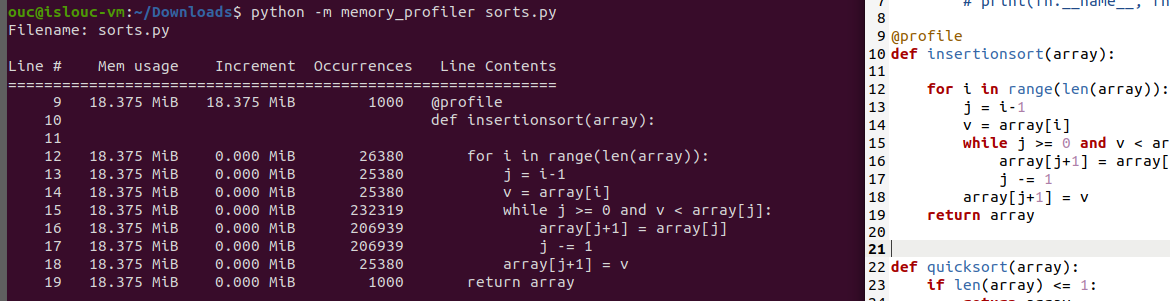
\includegraphics[width=1\textwidth]{006.jpg}
		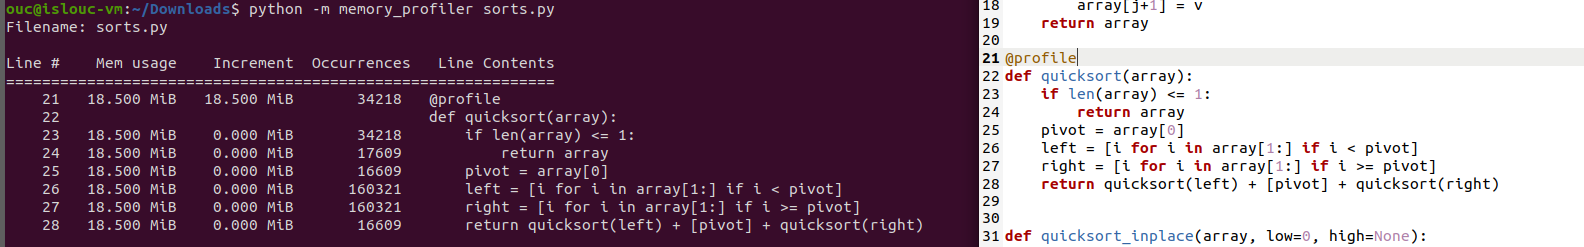
\includegraphics[width=1\textwidth]{007.jpg}
		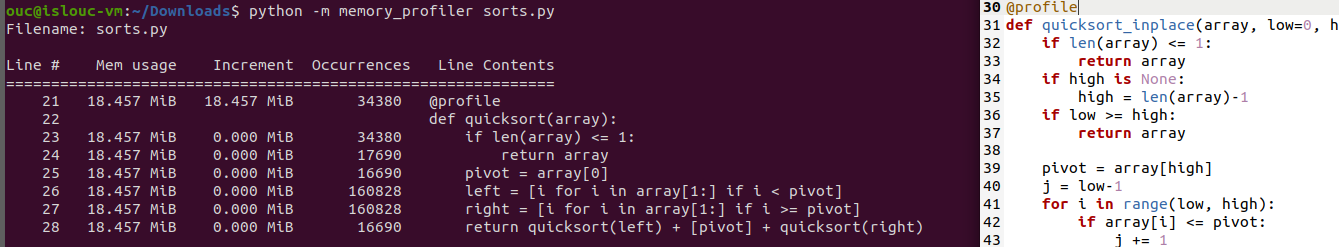
\includegraphics[width=1\textwidth]{008.jpg}
	\end{figure}
	
	由于test\_sorted用于测试的list太小了,插入排序和快速排序的内存占用相近。理论上插入排序占用的内存更小,因为插入排序的空间复杂度是 O(1),即它是原地排序,不需要额外的存储空间;而快速排序在递归过程中会使用到系统栈空间,其空间复杂度在平均情况下为 O(log n),最坏情况下为 O(n)。这种差异在处理大数据集时会变得更明显。
	
	\subsubsection{题目三}
	我们经常会遇到的情况是某个我们希望去监听的端口已经被其他进程占用了。让我们通过进程的 PID 查找相应的进程。首先执行 python -m http.server 4444 启动一个最简单的 web 服务器来监听 4444 端口。在另外一个终端中,执行 lsof | grep LISTEN 打印出所有监听端口的进程及相应的端口。找到对应的 PID 然后使用 kill <PID> 停止该进程。
	
	\paragraph{答:}
	结果如图。
		
	\begin{figure}[H]
		\centering
		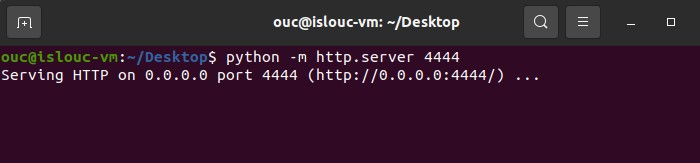
\includegraphics[width=1\textwidth]{009.jpg}
		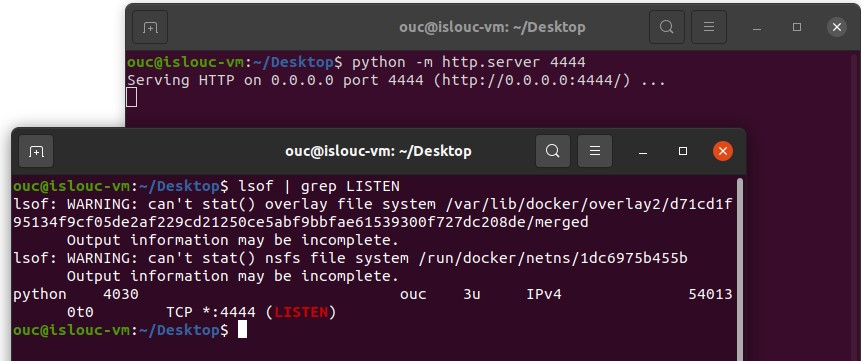
\includegraphics[width=1\textwidth]{010.jpg}
		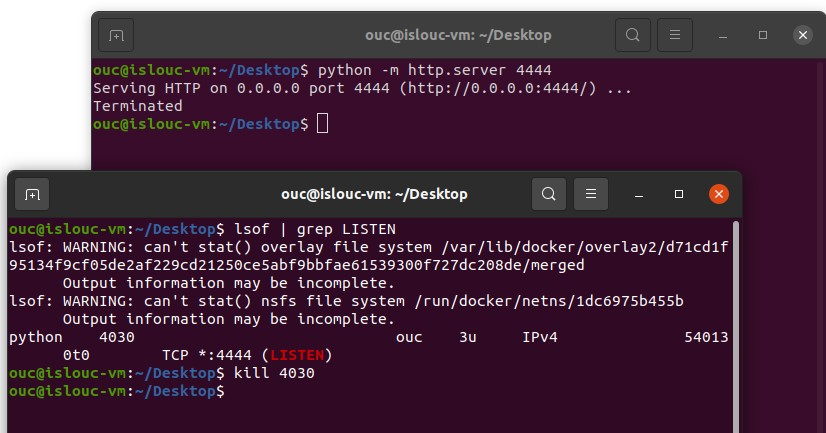
\includegraphics[width=1\textwidth]{011.jpg}
	\end{figure}
	
	\subsubsection{题目四}
	大多数的 makefiles 都提供了 一个名为 clean 的构建目标,这并不是说我们会生成一个名为 clean 的文件,而是我们可以使用它清理文件,让 make 重新构建。你可以理解为它的作用是“撤销”所有构建步骤。在上面的 makefile 中为 paper.pdf 实现一个 clean 目标。你需要将构建目标设置为 phony。
	
	\paragraph{答:}
	编写makefile,如下:
	
	\begin{figure}[H]
		\centering
		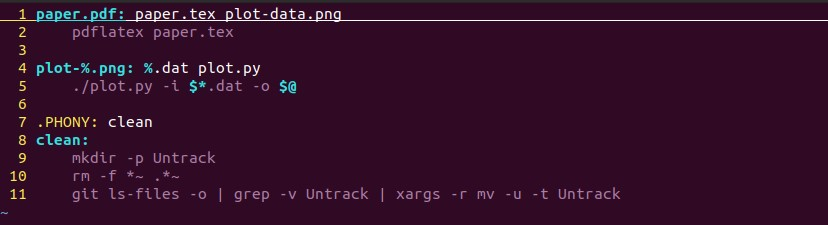
\includegraphics[width=1\textwidth]{012.jpg}
	\end{figure}
	
	将所有untracked文件移动到Untrack目录下,达到清理git仓库的目的。还需要设置git忽略该目录,用来放置untracked文件:
	
	\begin{figure}[H]
		\centering
		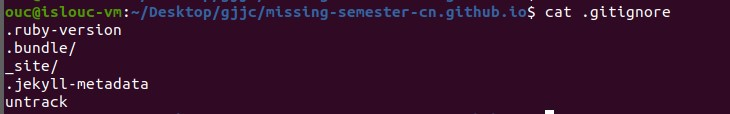
\includegraphics[width=1\textwidth]{013.jpg}
	\end{figure}
	
	结果如图:
	
	\begin{figure}[H]
		\centering
		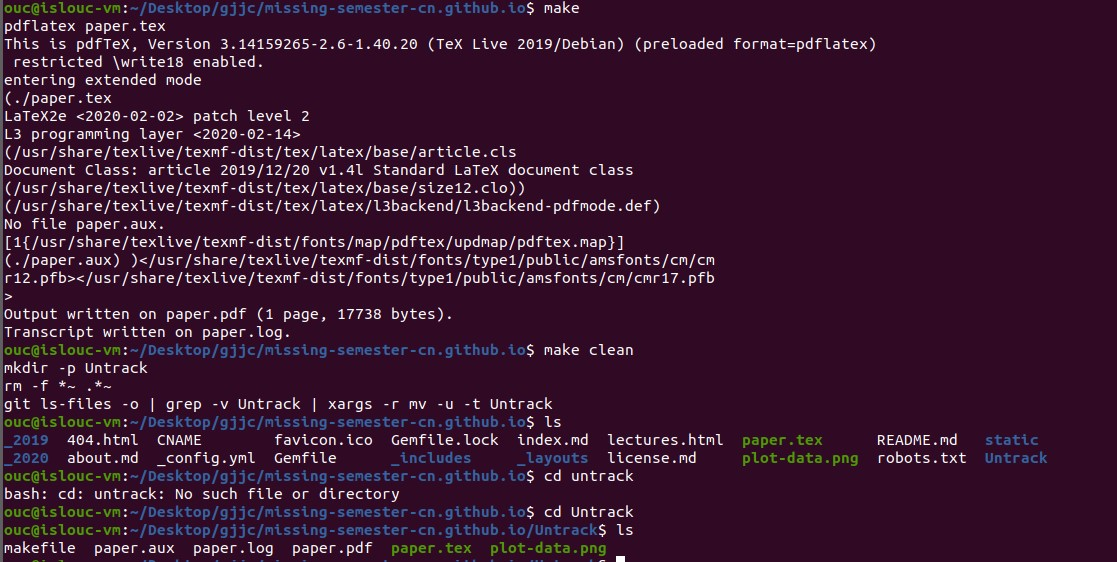
\includegraphics[width=1\textwidth]{014.jpg}
	\end{figure}
	
	\subsection{20个实例}
	
	\paragraph{(1)向系统日志中写日志:}
	使用 logger 并且如何找到能够将其存入系统日志的条目。
	
	
	\begin{figure}[H]
		\centering
		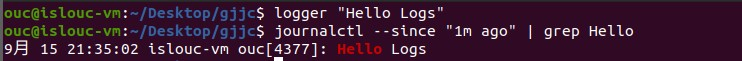
\includegraphics[width=1\textwidth]{015.jpg}
	\end{figure}
	
	\paragraph{(2)gdb:}
	disas命令查看反汇编代码。这里以bomb作为实例,gdb bomb, disas phase\_2 直接查看第2个炸弹执行函数的反汇编代码。
	
	\begin{figure}[H]
		\centering
		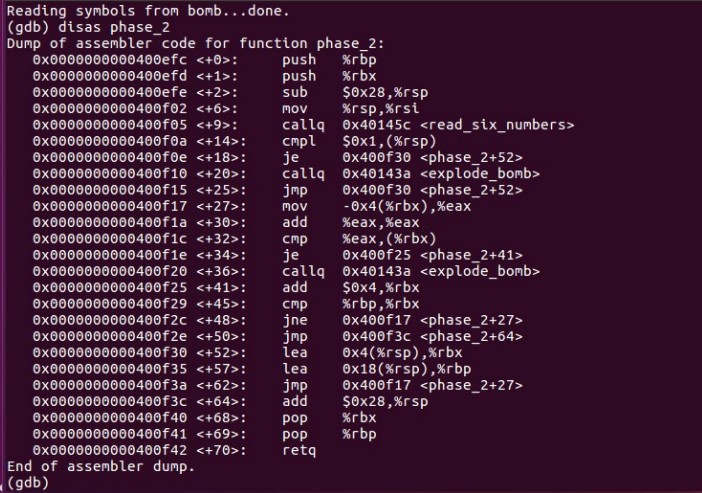
\includegraphics[width=1\textwidth]{016.jpg}
	\end{figure}
	
	\paragraph{(3)gdb:}
	在某一位置打断点并使程序运行到该断点处停止。这里以bomb作为实例,b read\_six\_numbers 在 read\_six\_numbers 函数入口处打上断点。 r 运行,程序运行到 read\_six\_number断点处自动停止。
	\begin{figure}[H]
		\centering
		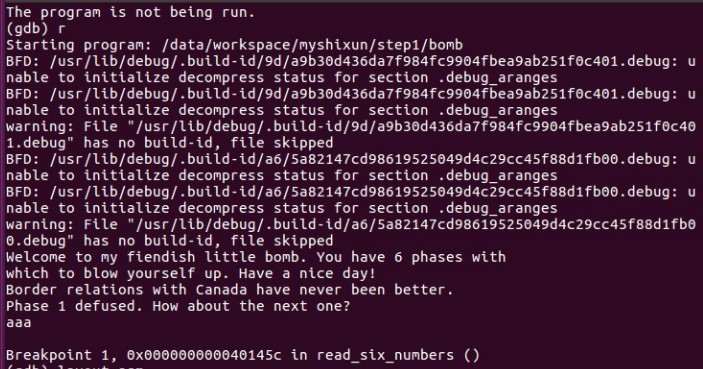
\includegraphics[width=1\textwidth]{017.jpg}
	\end{figure}
	
	\paragraph{(4)gdb:}
	输入指令 l (list),显示当前行的上、下若干行 C 语句的内容
	
	\begin{figure}[H]
		\centering
		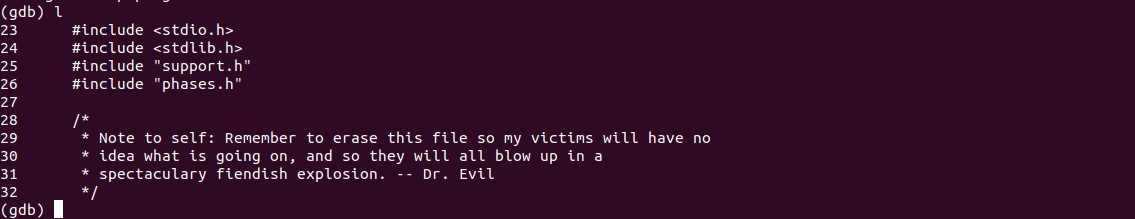
\includegraphics[width=1\textwidth]{019.jpg}
	\end{figure}
	
	
	\paragraph{(5)gdb:}
	 输入指令 n i/step i,时程序单步向前执行i条机器指令	
	
	
	\begin{figure}[H]
		\centering
		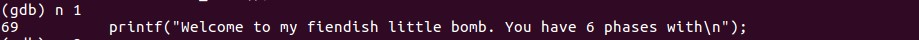
\includegraphics[width=1\textwidth]{018.jpg}
	\end{figure}
	
	\paragraph{(6)gdb:}	
	输入指令 n/step,单步执行 C 语句
	
	\begin{figure}[H]
		\centering
		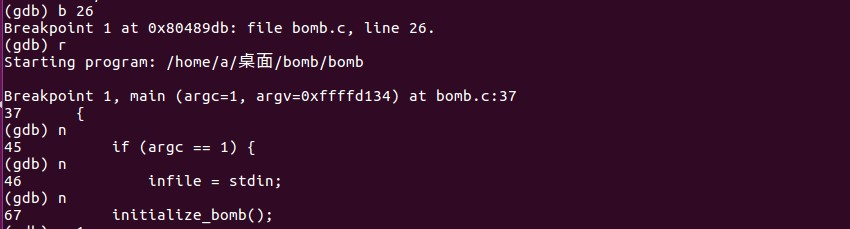
\includegraphics[width=1\textwidth]{020.jpg}
	\end{figure}
	
	\paragraph{(7)pwndbg:}
	安装pwndbg并进行调试。pwndbg在GDB的基础上,增加了针对二进制安全、漏洞利用和CTF挑战等特定场景的功能和命令,如ROP链构造、内存分析等。这里以逆向pwn文件game为例,文件已上传至github。这里在试图覆盖返回地址获取flag时出现了段错误,用pwndbg调试查看栈和报错信息,查找并加入合适的gadget后实现栈平衡,再次运行,成功获得了flag。
	
	\begin{figure}[H]
		\centering
		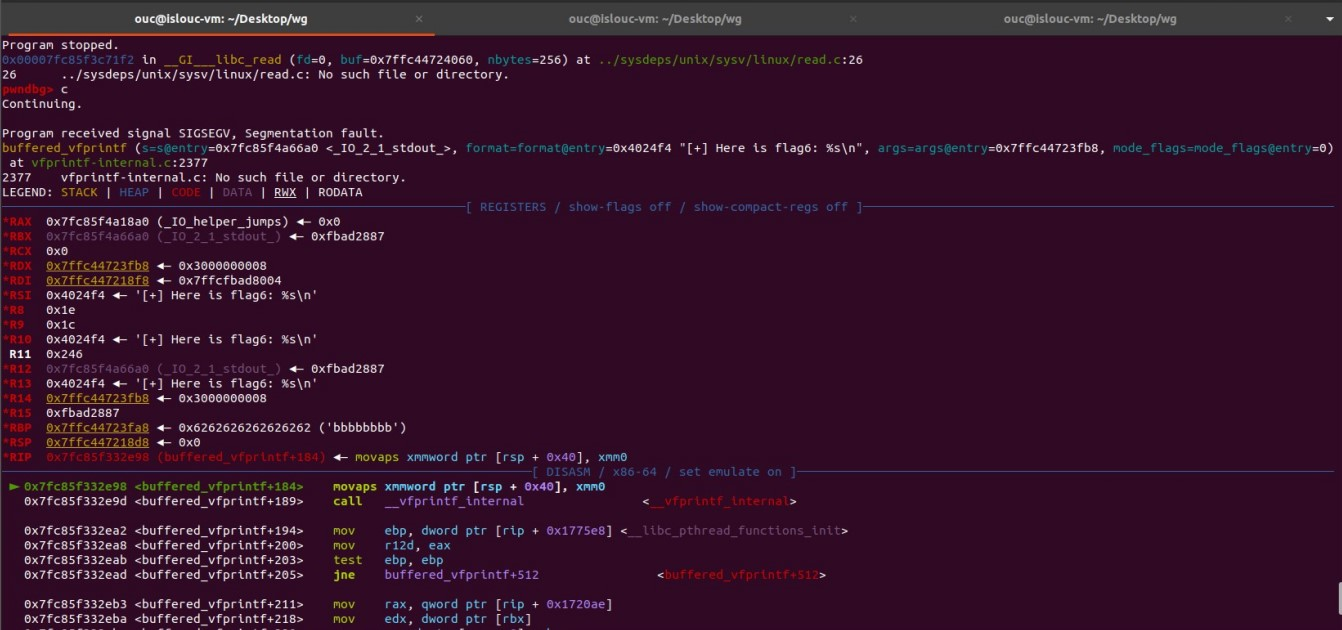
\includegraphics[width=1\textwidth]{021.jpg}
		
\includegraphics[width=1\textwidth]{022.jpg}
	\end{figure}
	
	\paragraph{(8)objdump 的使用:}
	使用 objdump 反汇编 bomb 得到汇编语言代码

	\paragraph{答:}
	objdump -d bomb > asm.txt
	
	“>”:重定向,将反汇编出来的源程序输出至 asm.txt 文件中.
	
	打开反汇编源代码文件
	
	gedit asm.txt
	
	\begin{figure}[H]
		\centering
		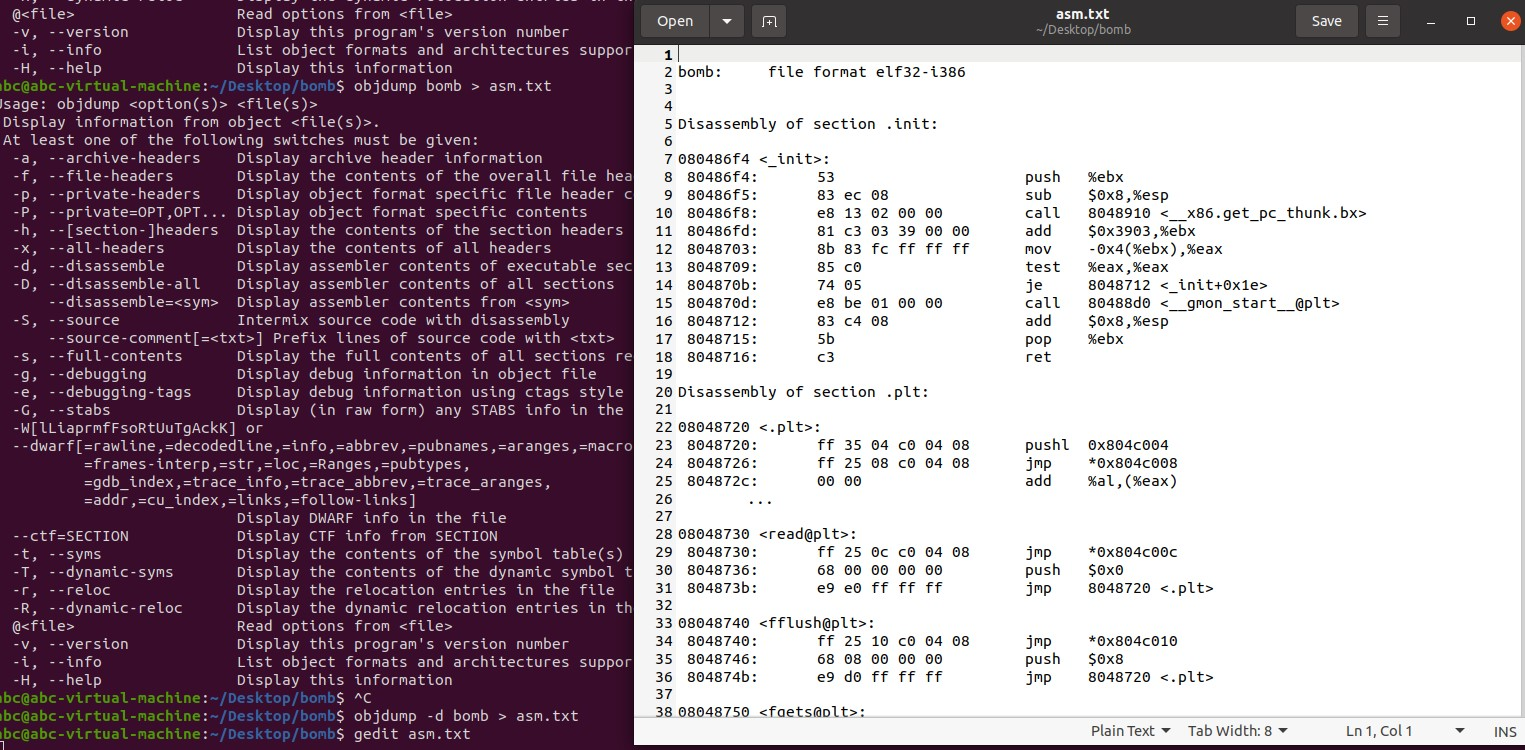
\includegraphics[width=1\textwidth]{039.jpg}
	\end{figure}
	
	\paragraph{(9)Wireshark:}
	Wireshark 这样的网络数据包分析工具可以帮助用户获取网络数据包的内容并基于不同的条件进行过滤。以you-got-me.pcapng为例,用wireshark分析,过滤http对象,文件列表中发现flag1.png,导出图片即得flag。文件已上传至github。
	
	\begin{figure}[H]
		\centering
		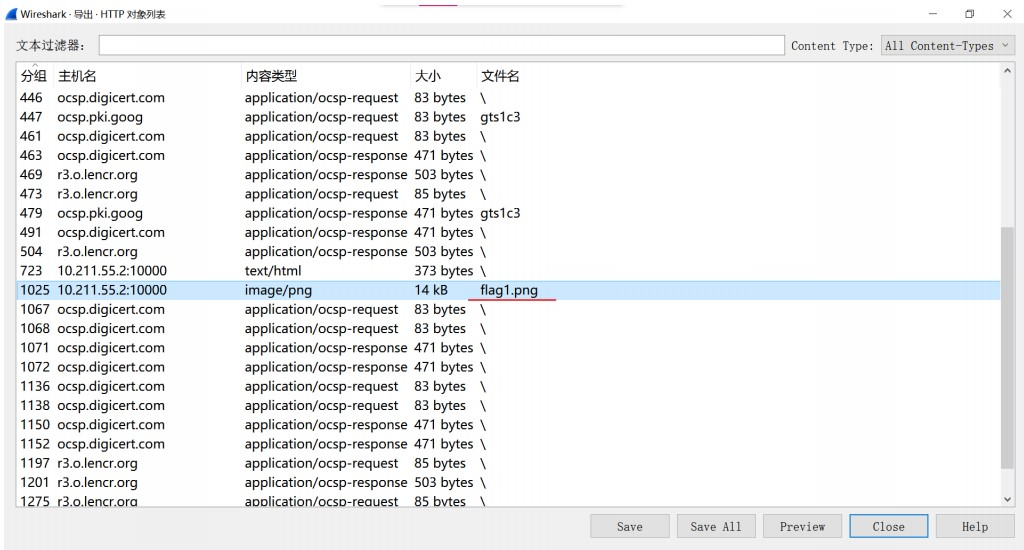
\includegraphics[width=1\textwidth]{023.jpg}
		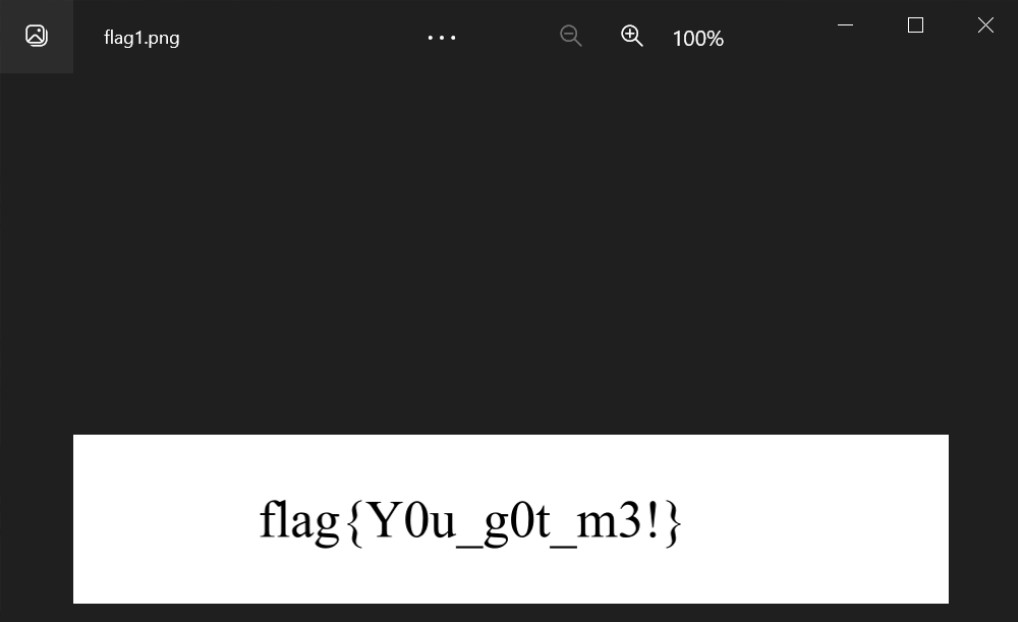
\includegraphics[width=1\textwidth]{024.jpg}
	\end{figure}
	
	\paragraph{10)性能分析-计时:}
	执行一个用于发起 HTTP 请求的命令,通过time命令查看该命令执行的CPU 内核时间、CPU 用户时间和真实时间,
	
	\begin{figure}[H]
		\centering
		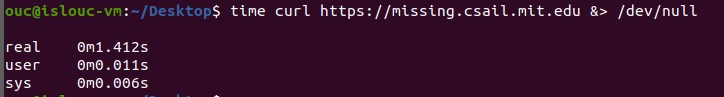
\includegraphics[width=1\textwidth]{025.jpg}
	\end{figure}
	
	\paragraph{(11)perf:}
	perf 可以报告不佳的缓存局部性(poor cache locality)、大量的页错误(page faults)或活锁(livelocks)。以sort.py为例,使用perf检查每个插入排序算法的循环次数、缓存命中和丢失。
	
	\begin{figure}[H]
		\centering
		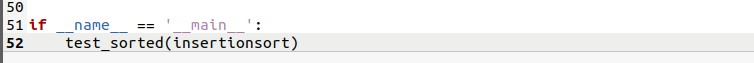
\includegraphics[width=1\textwidth]{026.jpg}
		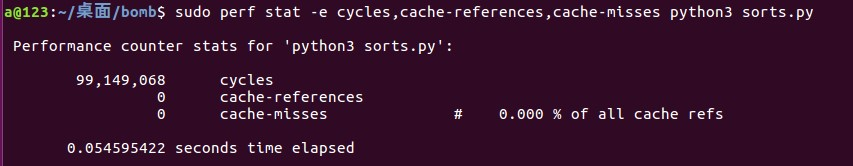
\includegraphics[width=1\textwidth]{027.jpg}
	\end{figure}
	
	\paragraph{(12)可视化:}
	这里有一些用于计算斐波那契数列 Python 代码,它为计算每个数字都定义了一个函数。将代码拷贝到文件中使其变为一个可执行的程序。首先安装 pycallgraph 和 graphviz。并使用 pycallgraph graphviz -- ./fib.py 来执行代码并查看 pycallgraph.png 这个文件。
	
	\begin{figure}[H]
		\centering
		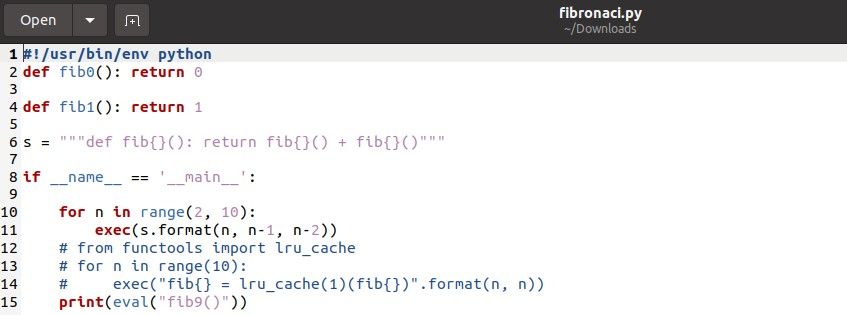
\includegraphics[width=1\textwidth]{028.jpg}
		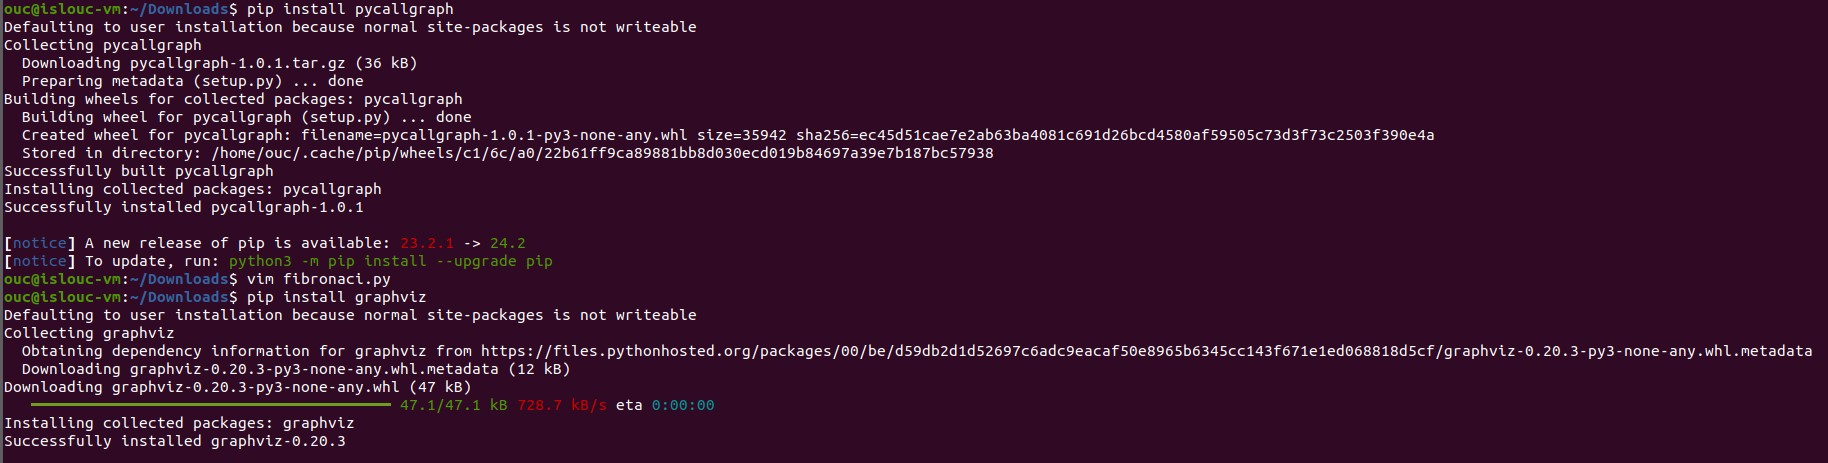
\includegraphics[width=1\textwidth]{030.jpg}
		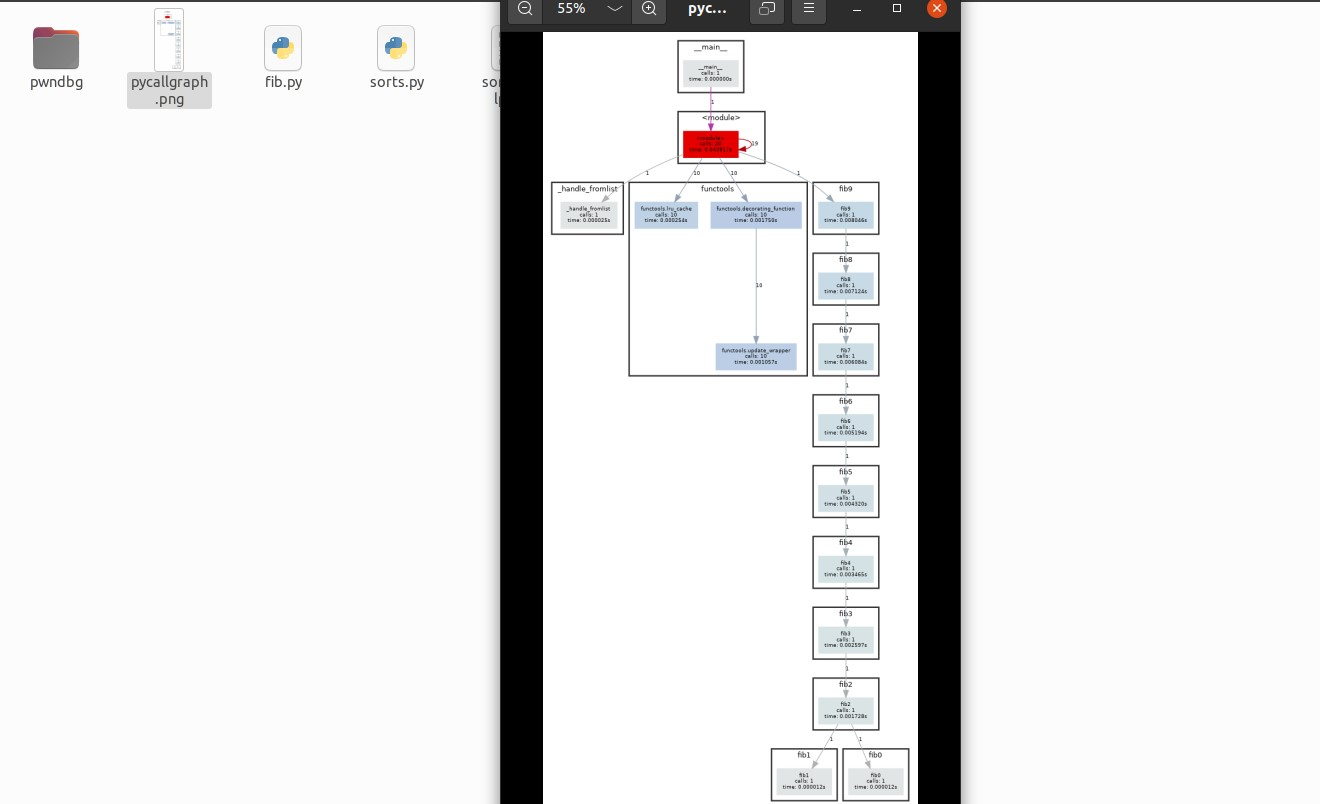
\includegraphics[width=1\textwidth]{031.jpg}
	\end{figure}
	
	\paragraph{(13)进程资源的可视化:}	
	限制进程资源也是一个非常有用的技术。执行 stress -c 3 创建负载并使用htop 对 CPU 消耗进行可视化。
	
	\begin{figure}[H]
		\centering
		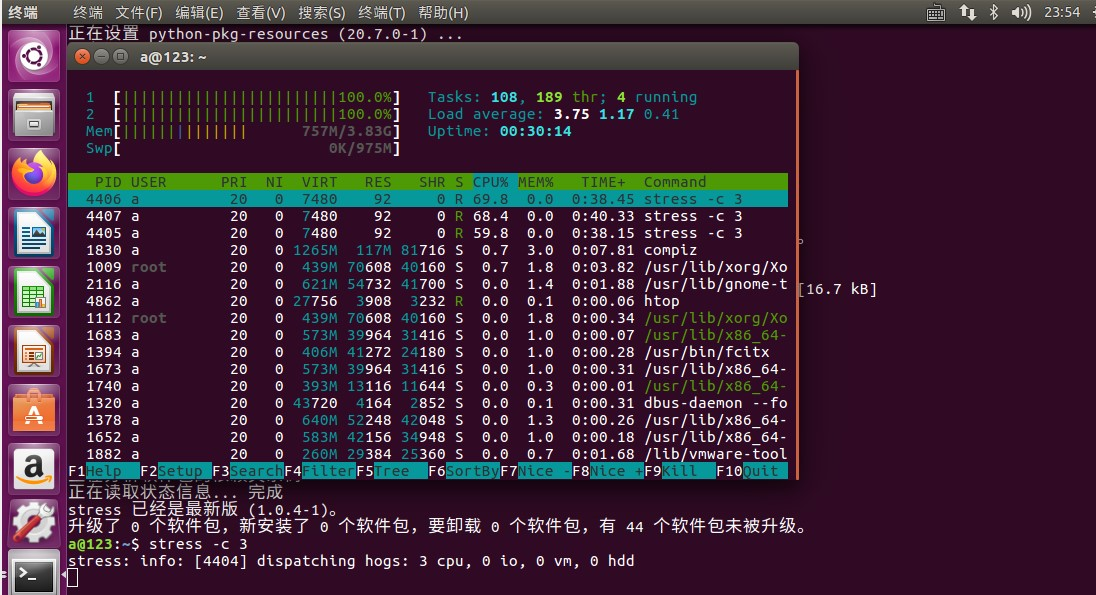
\includegraphics[width=1\textwidth]{032.jpg}
	\end{figure}
	
	\paragraph{(14)进程资源的可视化:}
	执行taskset --cpu-list 0,2 stress -c 3 限制资源消耗,并可视化。stress 占用了3个 CPU 吗?为什么没有?
	
	\paragraph{答:}
	运行taskset --cpu-list 0,2 stress -c 3时限制了stress进程只能在CPU 0和CPU 2上运行。也就是说,请求了3个CPU密集型任务,但只指定了两个可用的CPU核心。阅读man taskset可知,如果进程被限制在少于请求数量的CPU核心上,那么这些核心将尽可能平均地分担负载。但是,由于只有2个核心可用,所以实际上只有2个stress的CPU密集型任务能够并行运行。所以stress 没有占用3个 CPU 。
	
	\begin{figure}[H]
		\centering
		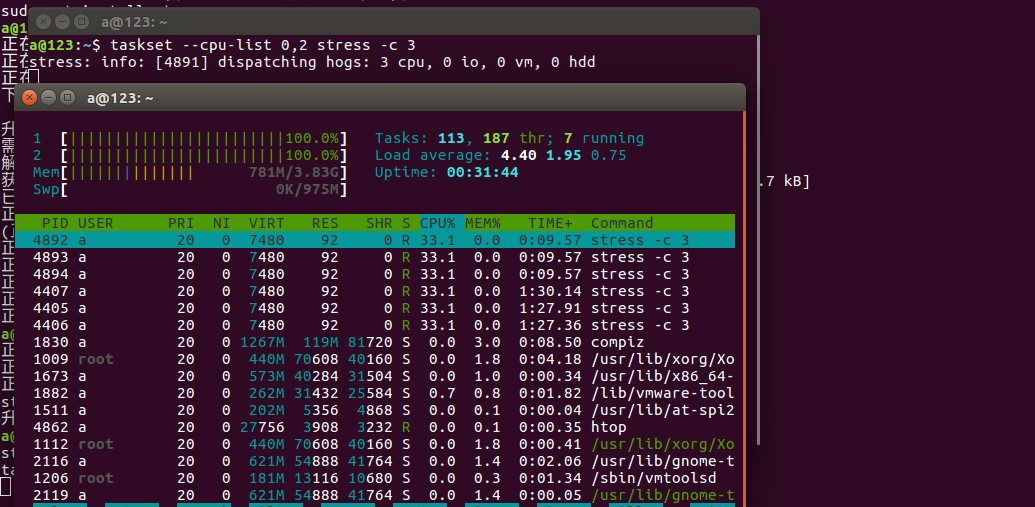
\includegraphics[width=1\textwidth]{033.jpg}
	\end{figure}
	
	\paragraph{(15)命令行标志参数:}
	使用 rm 删除一个叫 -r 的文件。
	
	\begin{figure}[H]
		\centering
		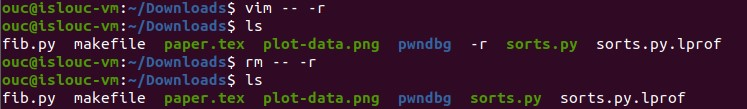
\includegraphics[width=1\textwidth]{029.jpg}
	\end{figure}
	
	\paragraph{(16)git:}
	Git 可以作为一个简单的 CI 系统来使用,在任何 git 仓库中的 .git/hooks 目录中,您可以找到一些文件(当前处于未激活状态),它们的作用和脚本一样,当某些事件发生时便可以自动执行。请编写一个 pre-commit 钩子,它会在提交前执行 make paper.pdf 并在出现构建失败的情况拒绝您的提交。
	
	\paragraph{答:}
	修改.git/hooks目录下面的pre-commit.sample文件,加入以下几行:
	if  ! make ; then
	
	echo "build failed, commit rejected"
	
	exit 1
	
	fi
	
	然后将其命名为pre-commit
	
	\begin{figure}[H]
		\centering
		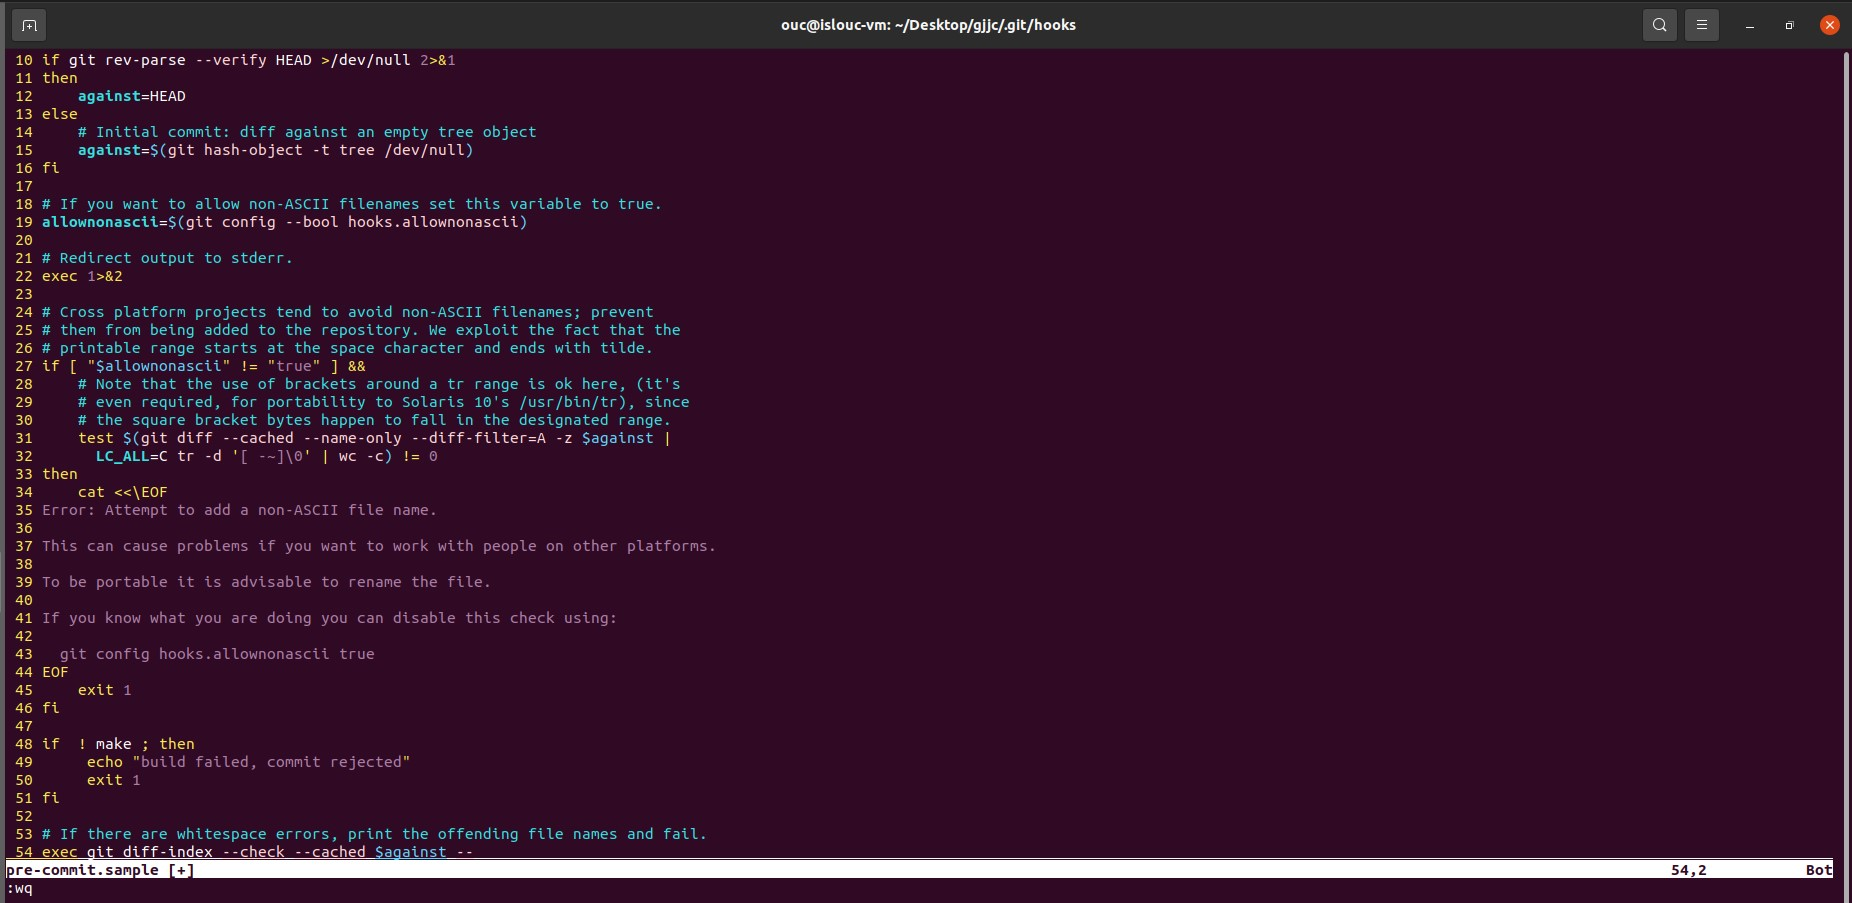
\includegraphics[width=1\textwidth]{034.jpg}
		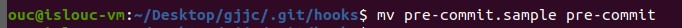
\includegraphics[width=1\textwidth]{035.jpg}
	\end{figure}
	
	\paragraph{(17)可读性:}
	以彩色文本显示终端信息时可读性更好。执行命令打印红色,测试用户的终端是否支持真彩色。
	
	\begin{figure}[H]
		\centering
		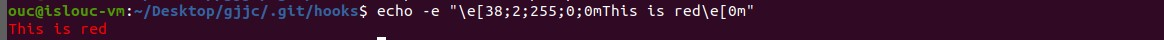
\includegraphics[width=1\textwidth]{036.jpg}
	\end{figure}
	
	\paragraph{(18)彩色文本:}	
	在终端中打印多种颜色。
	
	\paragraph{答:}
	编写脚本如下,运行脚本,查看终端的彩色输出。可以通过调整RGB值来获取输出文本的不同颜色。
	
	\begin{figure}[H]
		\centering
		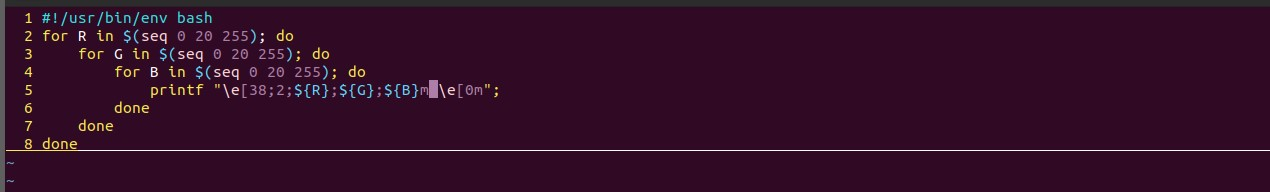
\includegraphics[width=1\textwidth]{037.jpg}
		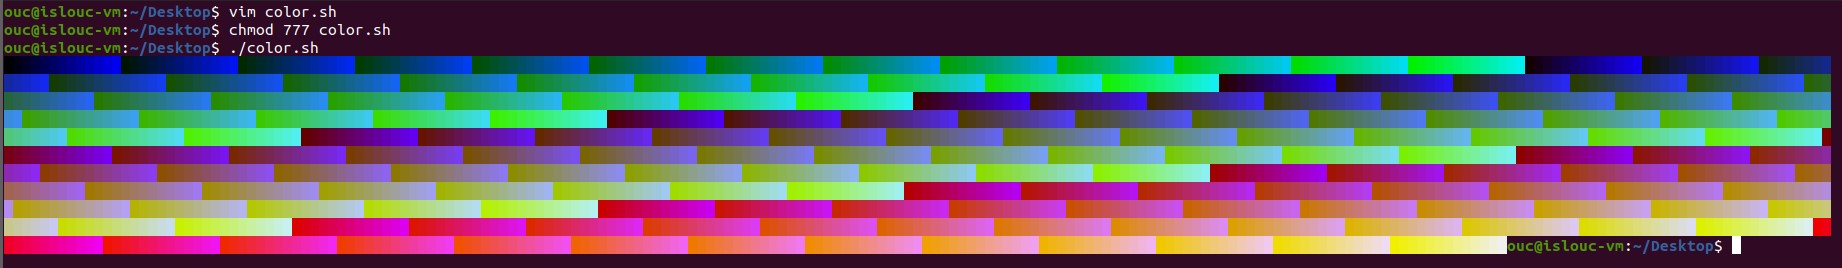
\includegraphics[width=1\textwidth]{038.jpg}
	\end{figure}
	
	\paragraph{(19)markdown:}
	安装markdown编写软件marktext并写一个文件,转成pdf格式。
	
	(文件已上传至github)

	\begin{figure}[H]
		\centering
		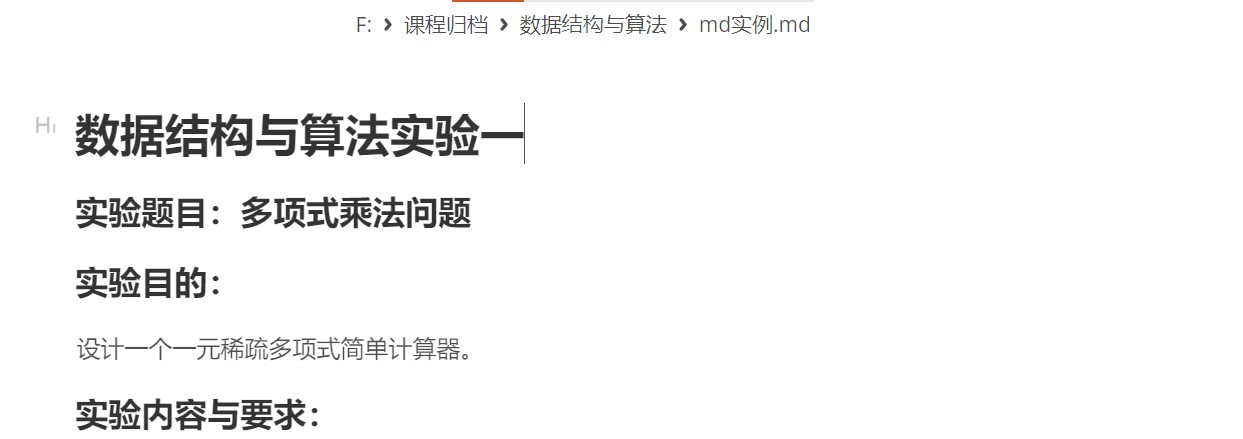
\includegraphics[width=1\textwidth]{096.jpg}
		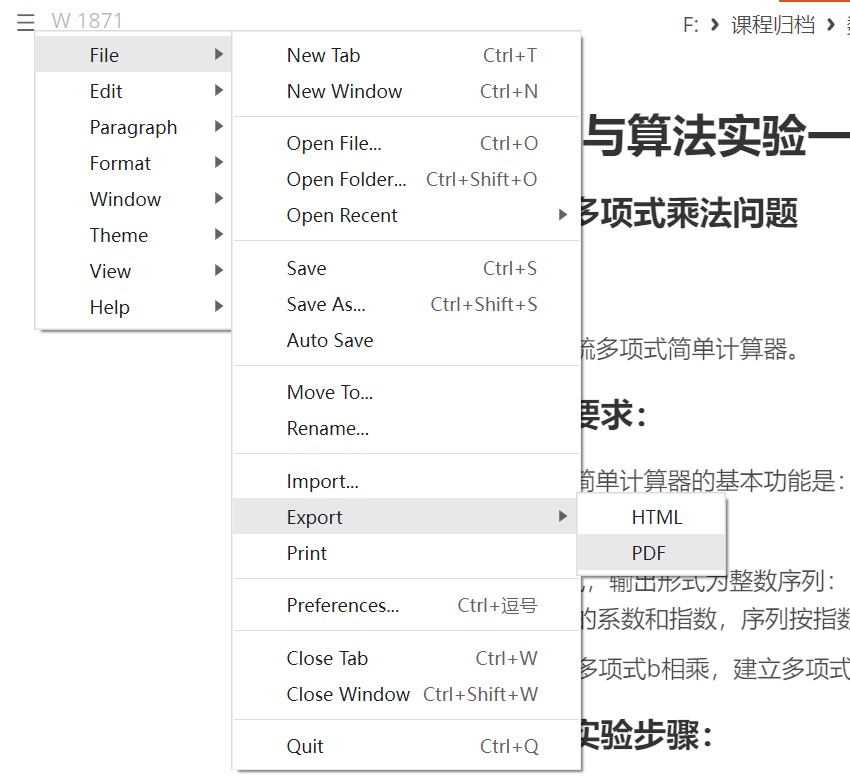
\includegraphics[width=1\textwidth]{095.jpg}
		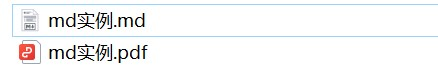
\includegraphics[width=1\textwidth]{097.jpg}
	\end{figure}
	
	\paragraph{(20)pytorch实例:}
	在pycharm写Python程序对图片进行 Sobel 算子卷积操作与空间域滤波。
	
	\paragraph{实例要求:}
	将 Sobel 算子编码到 pytorch 卷积核中,并用编码的卷积核对图像
	ori.jpg 执行卷积操作,输出结果(水平梯度图像、垂直梯度图像和梯度幅值图像),理解卷积操作与空间域滤波的关系。
	
	\paragraph{实例解答:}
	
	(1)加载图像,转换为灰度图像,方便创立 tensor 数据;升维,添加
	batch 维度。
	
	(2)定义 Sobel 算子的水平和垂直核,创建 PyTorch 卷积层,设置卷积核权重。
	
	(3)对图像应用水平和垂直 Sobel 滤波器得到水平梯度数据和垂直梯
	度数据;进一步计算梯度幅值图像。
	
	(4)将上一步数据更改到[0, 255]范围并转换为 uint8 类型,以便保存为图像文件。
	
	(5)保存结果。
	
	(具体代码及输出结果已上传至github库-task4-py0)
	
	\begin{figure}[H]
		\centering
		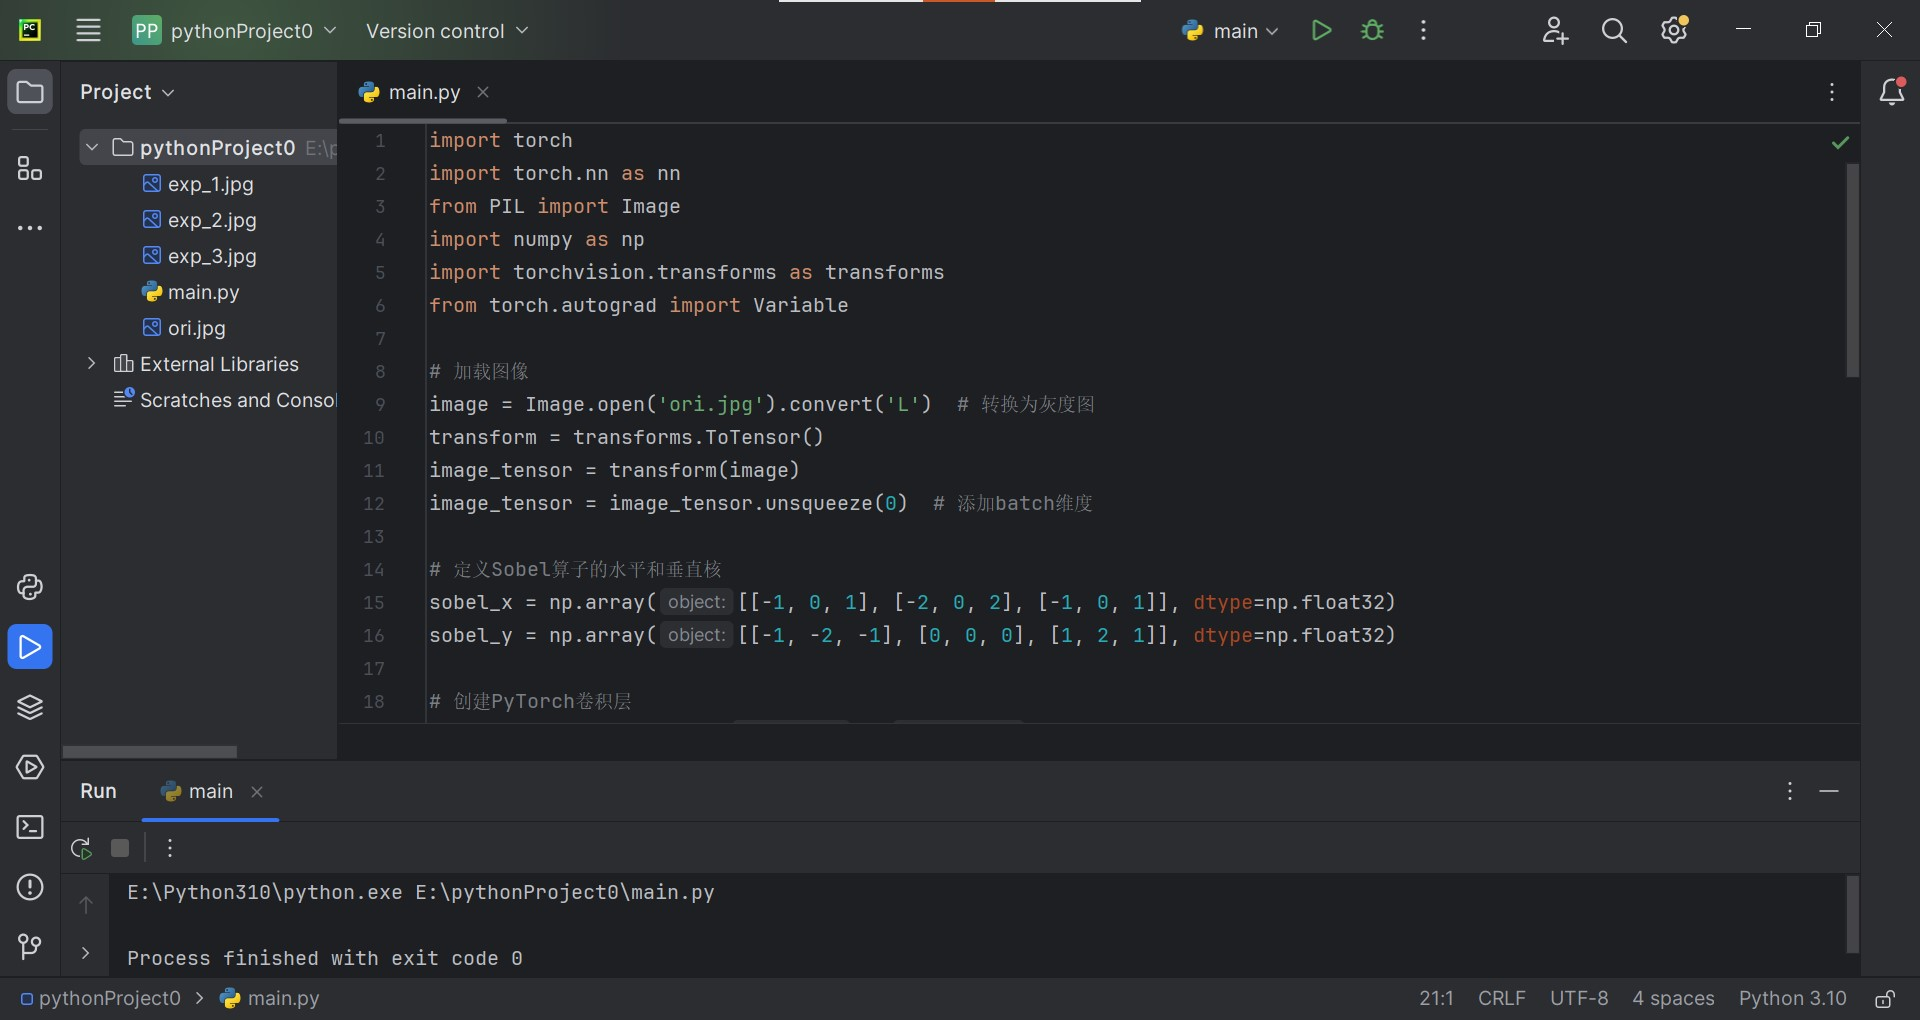
\includegraphics[width=1\textwidth]{098.jpg}
		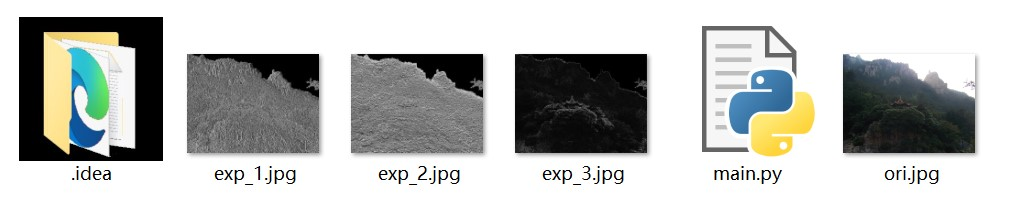
\includegraphics[width=1\textwidth]{099.jpg}
	\end{figure}
	
	\section{问题及解决方案}
	
	\paragraph{(1)}
	问题:运行perf时报错。
	
	\begin{figure}[h]
		\centering
		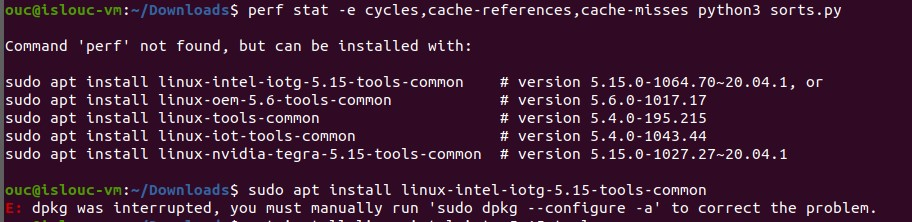
\includegraphics[width=1\textwidth]{100.jpg}
	\end{figure}
	
	解决方案:发现是之前装texlive时进程未完全完成安装便终止,故在运行并更新perf时遇到dpkg(Debian包管理器)配置未完成的问题。根据系统提示,手动运行sudo dpkg --configure -a来修正这个问题。(这一步耗费时间较长,后续直接换了虚拟机安装perf)
	
	\begin{figure}[h]
		\centering
		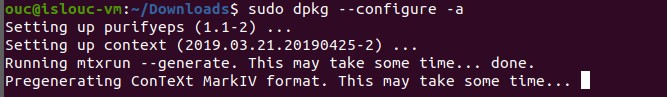
\includegraphics[width=1\textwidth]{101.jpg}
	\end{figure}
	
	\section{解题感悟}
	本实验中,通过练习调试及性能分析、元编程演示、大杂烩以及PyTorch的题目,我不仅学习到了Linux命令、各种性能分析工具以及调试工具的使用方法,还加深了对Python编程、系统资源管理及性能可视化分析的理解。本次实验的内容多而杂,对我们的综合素养和学习能力进行了锻炼,提高了我解决问题的能力。
	
	在实例中引用到了我之前学过的知识,温故而知新,让我又对这些工具的使用方法有了新的理解。在网络攻防先导实践课上使用过的pwndbg、wireshark和markdown,在计算机系统基础课上做bomb拆弹实验使用的gdb,在图像处理与分析课上做卷积相关程序使用的pytorch,在本实验中再次有所温习。除此之外也学到了不少新知识,比如git,cprofile等性能分析工具,perf等命令等。通过本次练习,我的综合素养得到了进一步的提升。
	
	\section{github链接}
	\underline{https://github.com/zxm2580/xtkfgjjc-202408.git}	
	
	\begin{figure}[H]
		\centering
		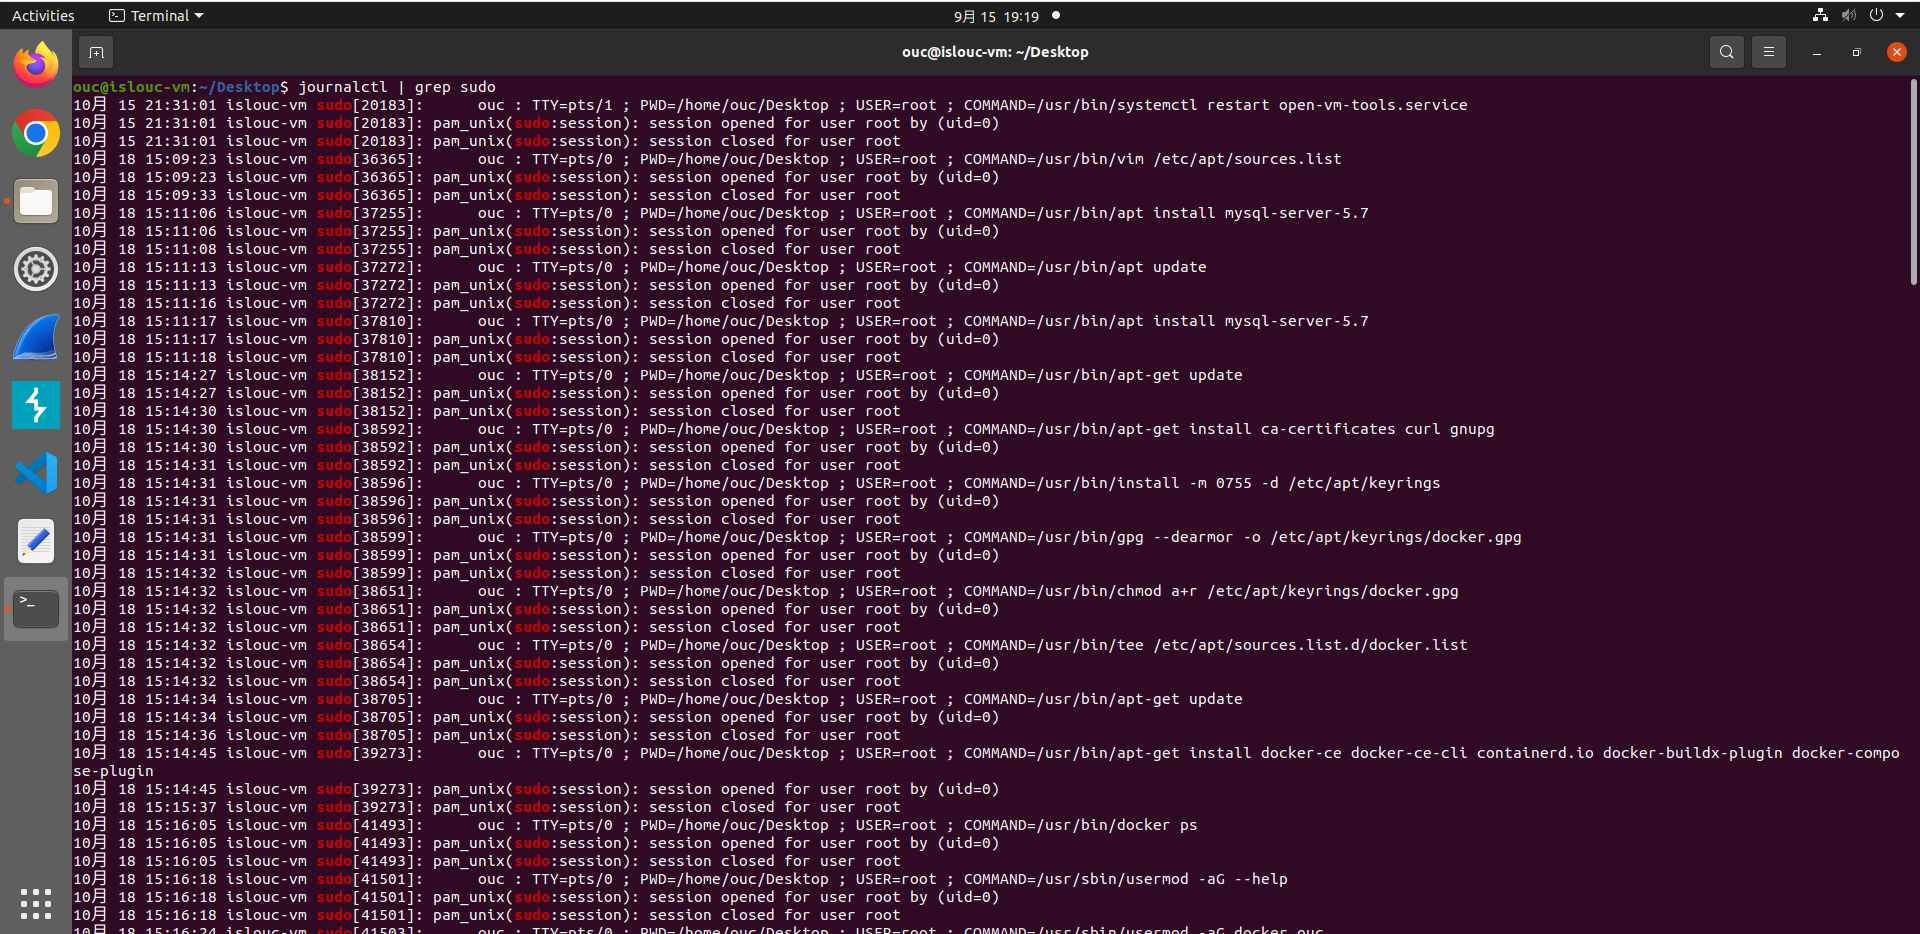
\includegraphics[width=1\textwidth]{001.jpg}
	\end{figure}
	
	
\end{document}